{\bf \normalsize (i) Tracking efficiency} - The tracking efficiency was calculated by obtaining the ratio between the yield at the reconstructed level and generated level, for a defined ``type" of particles (in our case non-identified particles) and it is estimated differentially in p$_T$, $\eta$, and z$_{vtx}$ of the event.\\

Tracking efficiency maps were produced as TH3D histograms (p$_T$, $\eta$, z$_{vtx}$) obtained from MC analysis on the minimum-bias samples LHC17f2b$\_$fast and LHC17f2b$\_$cent$\_$woSDD, and applying at reconstructed level the track selections (summarized in Table.~\ref{table:effCuts}). These efficiency maps were used in the analysis tasks to extract single track efficiencies; each correlation pairs found in the data analysis was inserted in correlation plots with a weight of {\bf 1/efficiency value}.  Plots of the $\pt$ dependence of the tracking efficiency for two different track selections are shown in Fig.~\ref{fig:trackeff}.

\begin{figure}[h]
	\centering
	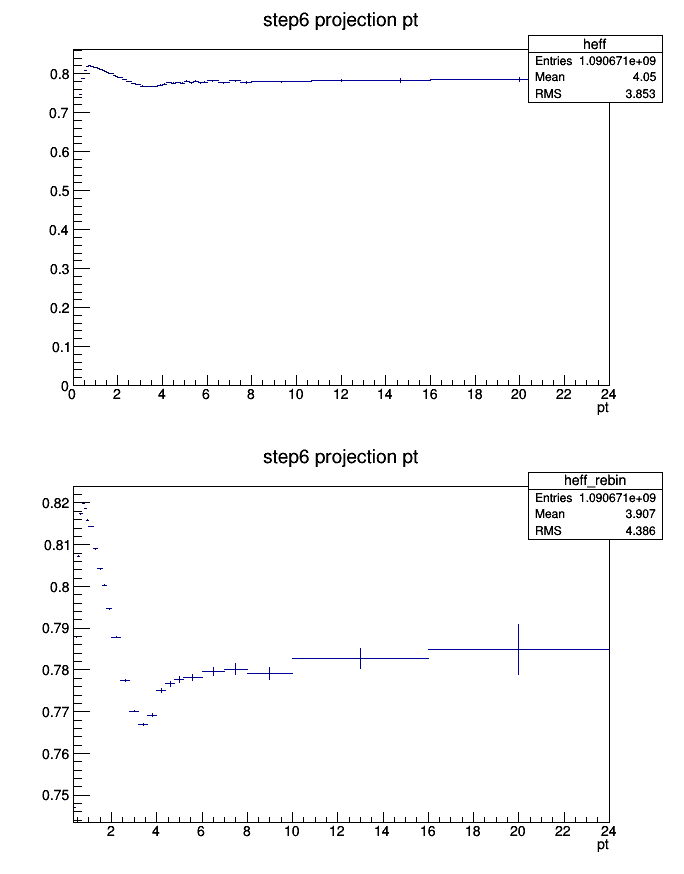
\includegraphics[scale=0.7]{figures/Effs/TrackEfficiency_pPb2016_defaultCuts.png}
    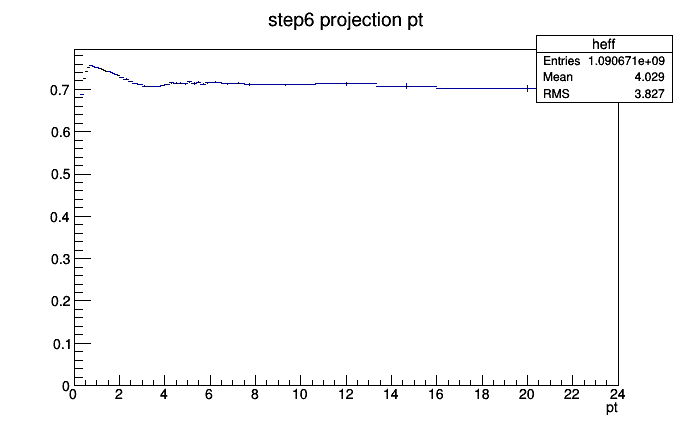
\includegraphics[scale=0.7]{figures/Effs/TrackEfficiency_pPb2016_Min3ITSCls.png}
	\caption{$p_T$ efficiency map for standard track selection (2 ITS clusters) on top panel, and alternate track selection, used for systematics (3 ITS clusters, filterbit4, ITS refit) on bottom panel.}
	\label{fig:trackeff}	
\end{figure}

\newpage
Details of cuts at event level and particle selection at different steps are listed in Table ~\ref{table:effCuts} . \\
\begin{table}[h]
\small
\centering % used for centering table

\begin{tabular}{  p{5cm} |  p{8.5cm} }
 \\
  \multirow{1}{*}{\large \textbf {MC Generated }} \\
\hline
\\
     Stages         &              Cuts \\
\hline\hline & \\		            	
  1.MC Part with Generated Cuts         &    {\textbf {After Event Selection}}\\
																		   & Charge\\
																		    & PDG Code\\
														  				  & Physical Primary \\

   2. MC Part with Kine Cuts         &              {\textbf {Kinematics Cuts }}\\
															    & -0.8$\textless \eta \textless  0.8$\\
															    & pT $\textgreater$ 0.3 (GeV/$c$)\\

&		\\            	


\multirow{1}{*}{\large \textbf {MC Reconstructed }} & \\
\hline


\hline & \\		            	                        	
4. Reco tracks        &                             {\textbf {After Event Selection}}\\
															   & Physical Primary \\
															
															
5. Reco tracks with Kine Cuts         &               {\textbf  {Kinematics Cuts }}\\
															    & -0.8$\textless \eta \textless  0.8$\\
															    & pT $\textgreater$ 0.3 (GeV/$c$)\\



6. MC true with Quality Cuts         &      			      {\textbf  {Quality Cuts }} \\
																	&SetRequireSigmaToVertex(kFALSE) \\
																	&SetDCAToVertex2D(kFALSE) \\
																	&SetMinNCrossedRowsTPC(70)\\
																	&SetMinRatioCrossedRowsOverFindableClustersTPC(0.8)\\
																	&SetMinNClustersITS(2)\\
																	&SetMaxChi2PerClusterTPC(4)\\
																	&SetMaxDCAToVertexZ(1) \\
																	&SetMaxDCAToVertexXY(1) \\
																	&SetRequireTPCRefit(TRUE) \\
																	&SetRequireITSRefit(FALSE) \\

7. Reco tracks with Quality Cuts         &             {\textbf  {Same as step 6}} \\

 &\\		            	            		

 \hline \hline
 \\
\end{tabular}
\caption{\large {Single Track Efficiency cuts detail}} % title of Table
\label{table:effCuts}	
\end{table}

{\bf \large (ii) D Meson efficiency} - Due to limited statistics, the correlation analysis is performed in quite wide p$_\mathrm{T}$ bins and in each of them the reconstruction and selection efficiency of D mesons is not flat, in particular in the lower $\pt$ region. We correct for the p$_\mathrm{T}$ dependence of the trigger efficiency within each p$_\mathrm{T}$-bin.

This correction is applied online, by using a map of D meson efficiency as a function of p$_\mathrm{T}$ and event multiplicity (in terms of SPD tracklets in $|\eta|<1$) extracted from the enriched Monte Carlo sample LHC17d2a$\_$fast$\_$new. The $\eta$ dependence was neglected due to the statistics of the available Monte Carlo sample, which avoided the possibility of performing a 3D study.

To properly count the number of trigger particles used to normalize the correlation distributions, $N_\text{trig}$, each D meson is weighted with the inverse of its efficiency
in the invariant mass distribution. The main role of the correction for the D meson efficiency is to account for the $\pt$ dependence of the correlation distribution within a given D meson $\pt$ interval. Indeed, only the $\pt$ shape of the D meson efficiency within the correlation $\pt^{\rm trig}$ ranges is relevant while the average value
in the $\pt$ range is simplified due to the normalization of the correlation distribution to the number of trigger particles.

It was observed that multiplicity dependence of the efficiency does not bias the extraction of the signal yield from the invariant mass distributions (which, as anticipated, are also weighted in the same manner). Efficiency plots for $\Dzero$, $\Dplus$ and $\Dstar$ mesons are shown in Figs.~\ref{fig:dEffPrompt} and ~\ref{fig:dEffFD}.

\begin{figure}[!htp]     %da c
	\centering
%Marianna
    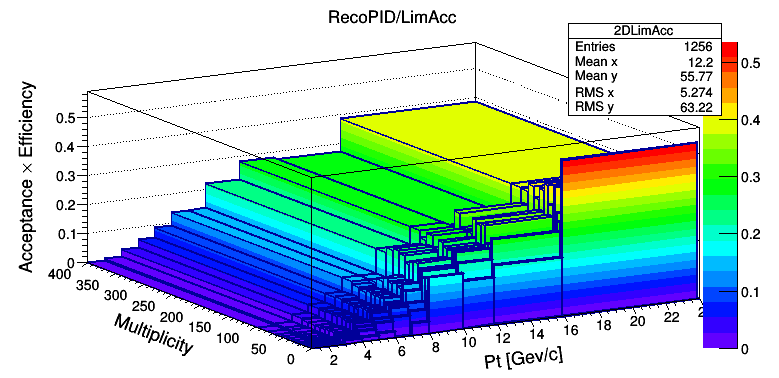
\includegraphics[width=.48\linewidth]{figures/Effs/EfficiencyMap_2D_DPlus_c_Ref_wLimAcc_Plot.png}
	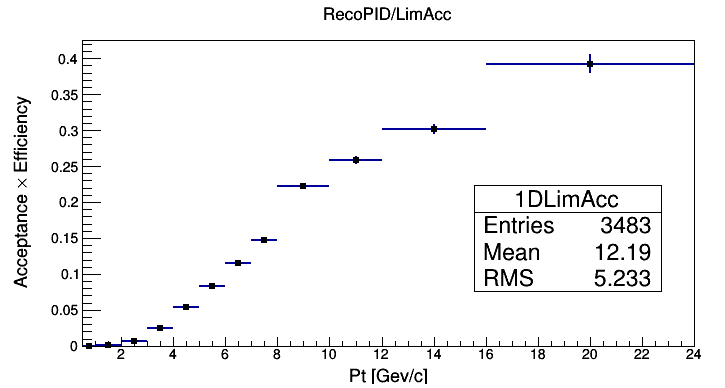
\includegraphics[width=.48\linewidth]{figures/Effs/EfficiencyMap_1D_DPlus_c_Ref_wLimAcc_Plot.png}  % by Fabio
	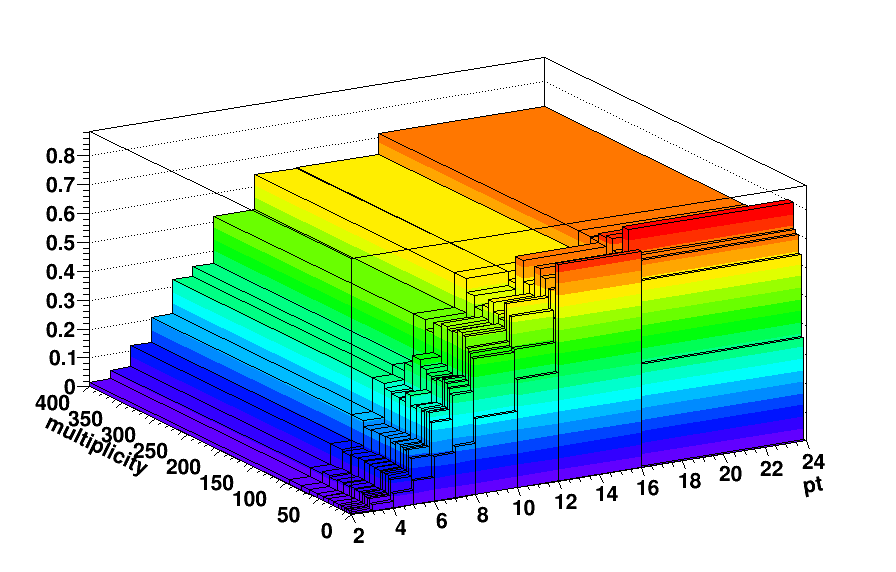
\includegraphics[width=.48\linewidth]{figures/Effs/EfficiencyMap_2D_DStar_c_Ref_wLimAcc_Plot.png}
	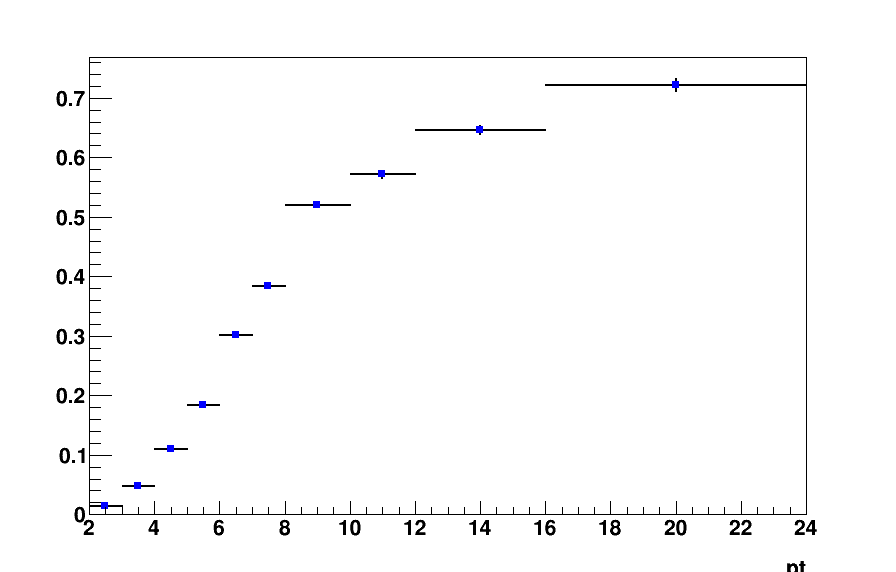
\includegraphics[width=.48\linewidth]{figures/Effs/EfficiencyMap_1D_DStar_c_Ref_wLimAcc_Plot.png}  % by Fabio
	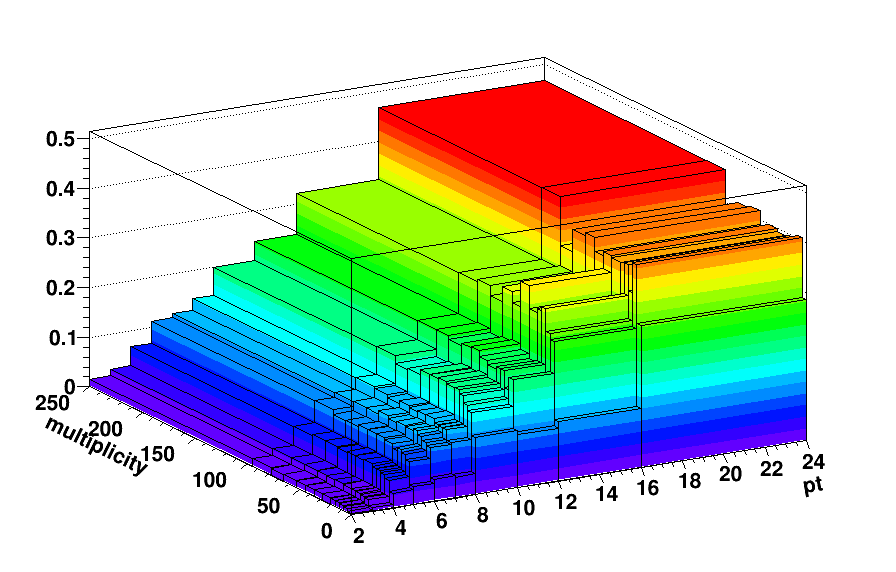
\includegraphics[width=.48\linewidth]{figures/Effs/EfficiencyMap_2D_Dzero_c_Ref_wLimAcc_Plot.png}
	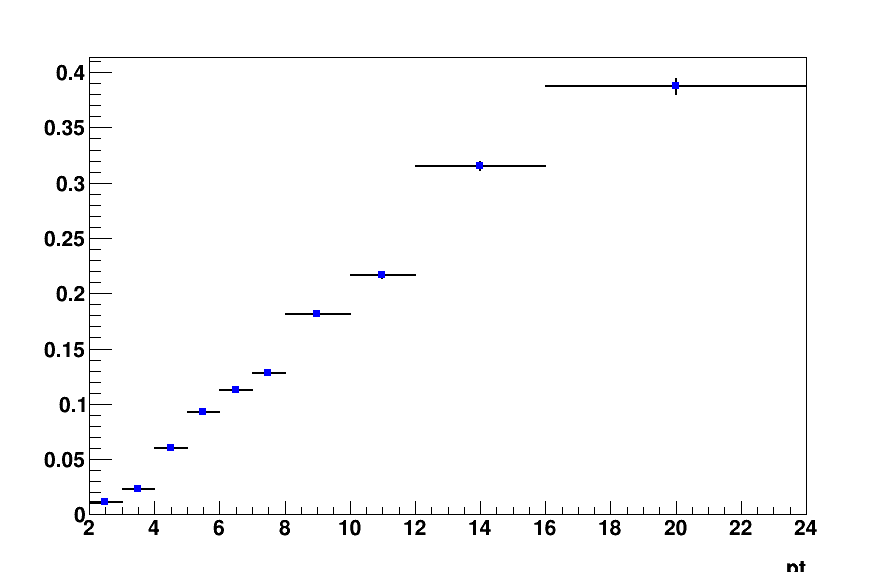
\includegraphics[width=.48\linewidth]{figures/Effs/EfficiencyMap_1D_Dzero_c_Ref_wLimAcc_Plot.png}  % by Fabio
	
	%\includegraphics[width=.30\linewidth]{figures/D0Eff_ProjMult_3to4GeV.png}
	%\includegraphics[width=.30\linewidth]{figures/D0Eff_ProjMult_5to6GeV.png}
	%\includegraphics[width=.30\linewidth]{figures/D0Eff_ProjMult_8to12GeV.png}
\caption{Top panel: (p$_\mathrm{T}$, multiplicity) dependence (left) and p$_T$ dependence (right) of prompt $D^{+}$ meson efficiency.
Mid panel: (p$_\mathrm{T}$, multiplicity) dependence (left) and p$_T$ dependence (right) of prompt $D^{*+}$ meson efficiency.
Bottom panel: (p$_\mathrm{T}$, multiplicity) dependence (left) and p$_T$ dependence (right) of prompt $D^{0}$ meson efficiency.
%s: multiplicity dependence of $D^0$ meson efficiency for three $D^0$ p$_\mathrm{T}$ ranges: 3-4 GeV/$c$ (left), 5-6 GeV/$c$ (center), 8-12 GeV/$c$ (right). For tracklet multiplicity$>$ 120, due to the limited statistics, the efficiency value is fixed to the one obtained for 90$<$tracklet multiplicity$<$120.
}
	\label{fig:dEffPrompt}	
\end{figure}

\begin{figure}[h]   %da B
	\centering
	%Marianna
		  % by Fabio
	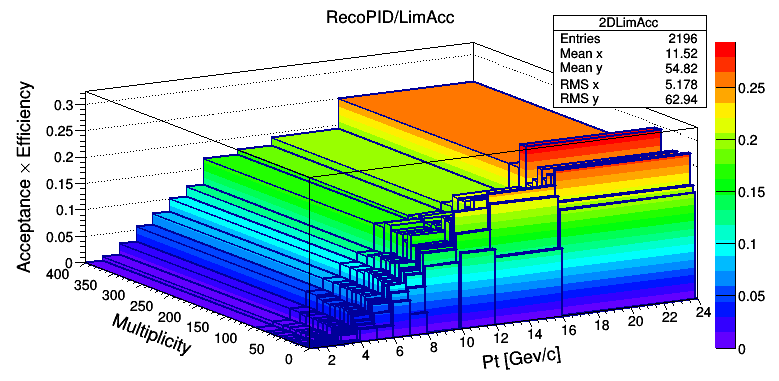
\includegraphics[width=.48\linewidth]{figures/Effs/EfficiencyMap_2D_DPlus_b_Ref_wLimAcc_Plot.png}
	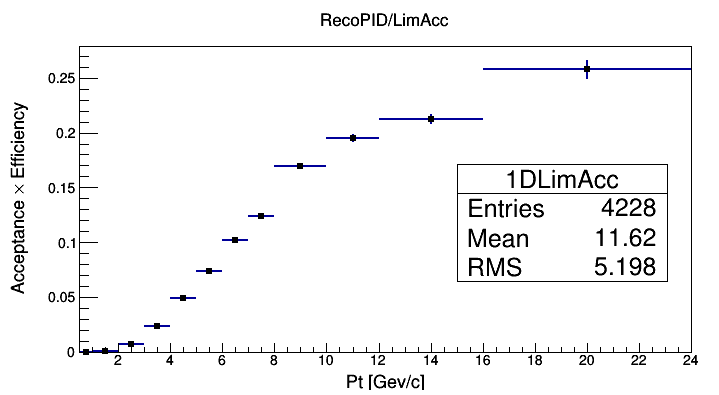
\includegraphics[width=.48\linewidth]{figures/Effs/EfficiencyMap_1D_DPlus_b_Ref_wLimAcc_Plot.png}
	  % by Fabio
	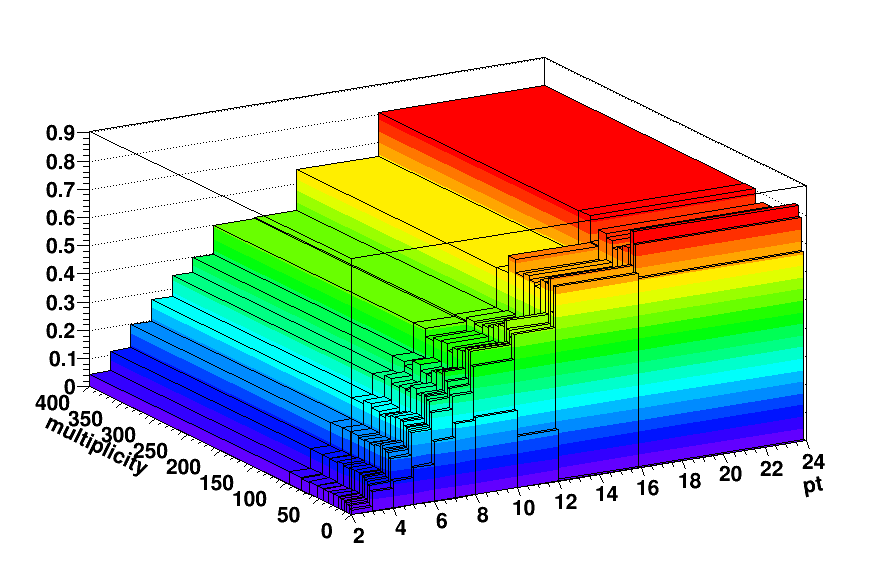
\includegraphics[width=.48\linewidth]{figures/Effs/EfficiencyMap_2D_DStar_b_Ref_wLimAcc_Plot.png}
	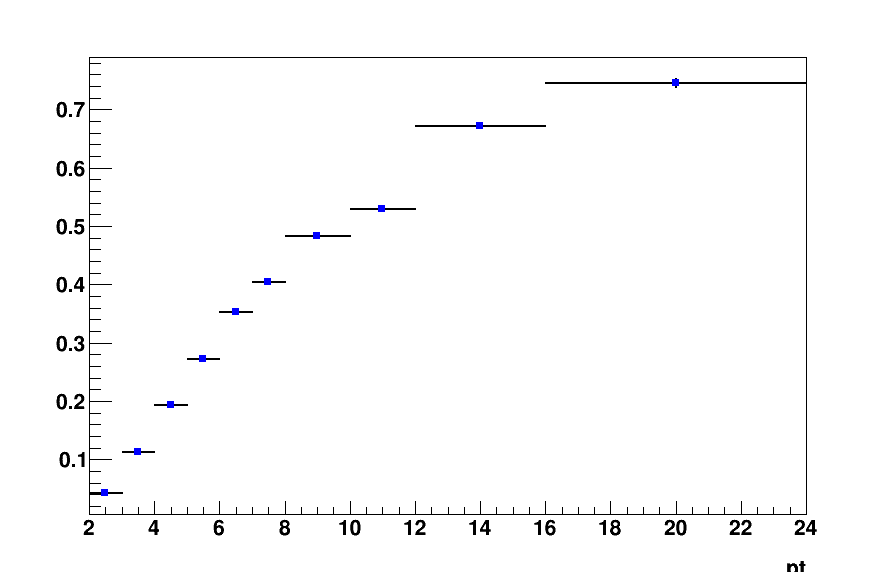
\includegraphics[width=.48\linewidth]{figures/Effs/EfficiencyMap_1D_DStar_b_Ref_wLimAcc_Plot.png}
	  % by Fabio
	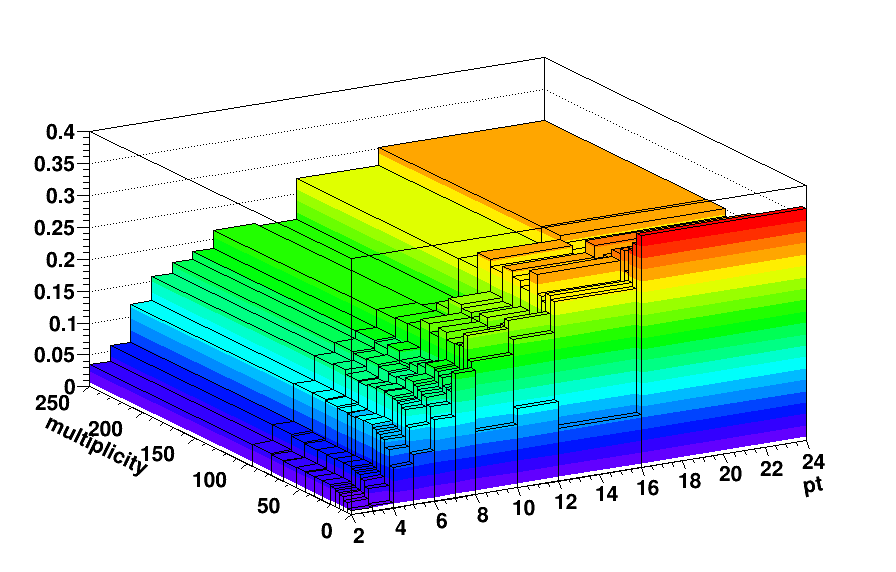
\includegraphics[width=.48\linewidth]{figures/Effs/EfficiencyMap_2D_Dzero_b_Ref_wLimAcc_Plot.png}
	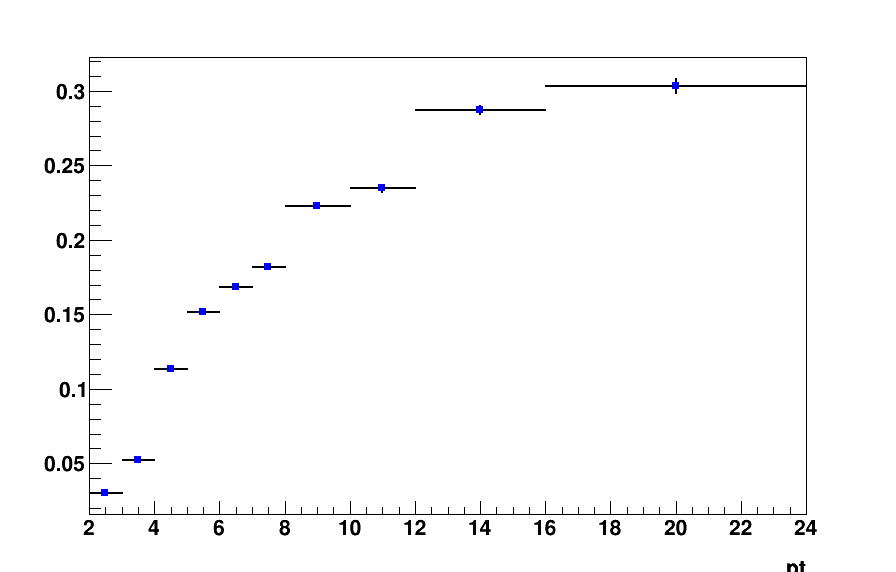
\includegraphics[width=.48\linewidth]{figures/Effs/EfficiencyMap_1D_Dzero_b_Ref_wLimAcc_Plot.png}
	\caption{Top panel: (p$_\mathrm{T}$, multiplicity) dependence (left) and p$_T$ dependence (right) of feed-down $D^{+}$ meson efficiency.
Mid panel: (p$_\mathrm{T}$, multiplicity) dependence (left) and p$_T$ dependence (right) of feed-down $D^{*+}$ meson efficiency.
Bottom panel: (p$_\mathrm{T}$, multiplicity) dependence (left) and p$_T$ dependence (right) of feed-down $D^{0}$ meson efficiency.}
	\label{fig:dEffFD}	
\end{figure}
\clearpage
%\begin{figure}[!htp]
	%\centering
%Marianna
	%\includegraphics[width=.48\linewidth]{figures/D0Eff_From_c_wLimAcc_2D_pPb.png}  % by Fabio
	%\includegraphics[width=.48\linewidth]{figures/D0Eff_From_c_wLimAcc_1D_pPb.png} \\
	%\includegraphics[width=.30\linewidth]{figures/D0Eff_ProjMult_3to4GeV.png}
	%\includegraphics[width=.30\linewidth]{figures/D0Eff_ProjMult_5to6GeV.png}
	%\includegraphics[width=.30\linewidth]{figures/D0Eff_ProjMult_8to12GeV.png}
%\caption{Top panel: (p$_\mathrm{T}$, multiplicity) dependence (left) and p$_T$ dependence (right) of prompt $\Dstar$ meson efficiency. Bottom panels: multiplicity dependence of $\Dstar$ meson efficiency for three $\Dstar$ p$_\mathrm{T}$ ranges: 3-4 GeV/$c$ (left), 5-6 GeV/$c$ (center), 8-12 GeV/$c$ (right). For tracklet multiplicity$>$ 120, due to the limited statistics, the efficiency value is fixed to the one obtained for 90$<$tracklet multiplicity$<$120.}
%	\label{fig:dstareff}	
%\end{figure}
%\newpage
